% ------------------------------------
% UNIVERSIDAD DE COSTA RICA
% Facultad de Ingeniería
% Escuela de Ingeniería Eléctrica
% IE0599 - Anteproyecto de Trabajo Final de Graduación
% By José Martínez Hdez, B34024
%
% PLANTILLA Y GUÍA DEL TRABAJO ESCRITO
% Versión: v1.0 (marzo 2017)
% ------------------------------------

% Tipo de documento
\documentclass[12pt,final]{proyectoelectrico}
\rmfamily
% A. PAQUETES Y MACROS ESPECIALES -------
% Paquetes y definiciones que no están incluidos 
% en la clase proyectoelectrico.cls o que son 
% propios del proyecto.
% -----------------------------------------
% OTROS PAQUETES E INSTRUCCIONES ESPECIALES
% -----------------------------------------

% PAQUETES
%%%%%%%%%%

% Para insertar PDFs
\usepackage{pdfpages}

% Para insertar código fuente estilizado
\usepackage{listings}
	\lstset{basicstyle=\ttfamily,
    		breaklines=true,
            numbers=left, 
    		numberstyle=\tiny, 
    		stepnumber=1, 
    		numbersep=6pt
            }
            
\usepackage{minted}

% Para usar múltiples columnas
\usepackage{multicol}

% Para crear árboles conceptuales
\usepackage{forest}

% Para insertar símbolos extraños
\usepackage{marvosym}

% Para insertar texto fútil
\usepackage{lipsum}

% NUEVAS INSTRUCCIONES
%%%%%%%%%%%%%%%%%%%%%%

\newcommand{\EIEx}{\textsc{Escuela \Lightning~ Ingeniería Eléctrica}}

% Definición de algunos símbolos matemáticos
\newcommand{\me}{\mathrm{e}}
\newcommand{\mi}{\mathrm{i}}
\newcommand{\mj}{\mathrm{j}}
\newcommand{\md}{\mathrm{d}}

% Listas con menos espacio entre ítemes (más ajustado)
\newcommand{\ajustado}{\itemsep0pt\parskip0pt\parsep0pt}

% FORMATO PARA EL REGLAMENTO
%%%%%%%%%%%%%%%%%%%%%%%%%%%%

\newcounter{articulo}
\newcommand{\articulo}[2]{
	{
    \stepcounter{articulo}
    \noindent
	\textbf{Artículo \thearticulo} --- \textit{#1}
	\vspace{2mm}\\
	}{
	#2
	\vspace{2mm} \\
	}
}

\newcounter{capitulo}
\newcommand{\capitulo}[1]{
	{
    \stepcounter{capitulo}
    \centering\large\bfseries
    Capítulo \Roman{capitulo}. #1
    \vspace{4mm}\\
    }
}

% Tipografía
\usepackage{libertine}
\usepackage{libertinust1math}
\usepackage[T1]{fontenc}
\renewcommand*{\ttdefault}{cmtt}

%%%AGREGADOS
\usepackage{multirow} % para las tablas
\definecolor{bl}{rgb}{0.6602, 0.796875, 0.8862}
\definecolor{cl}{rgb}{0.8359, 0.9140625, 0.96875}
\definecolor{bg}{rgb}{0.95,0.95,0.95}
\definecolor{p1}{rgb}{1.0,0.698,0.4}
\usetikzlibrary{shadows,arrows.meta}
\usepackage{adjustbox}
\usepackage{color}
\usepackage{graphicx}
\usepackage{epsfig}
\usepackage{multirow}
\usepackage{colortbl}
\definecolor{lightgray}{gray}{0.9}
\definecolor{bg1}{rgb}{0.8,1.0,0.8}
\usetikzlibrary{arrows.meta, shapes.geometric, calc, shadows}
\colorlet{mygreen}{green!75!black}
\colorlet{col1in}{red!30}
\colorlet{col1out}{red!40}
\colorlet{col2in}{mygreen!40}
\colorlet{col2out}{mygreen!50}
\colorlet{col3in}{blue!30}
\colorlet{col3out}{blue!40}
\colorlet{col4in}{mygreen!20}
\colorlet{col4out}{mygreen!30}
\colorlet{col5in}{blue!10}
\colorlet{col5out}{blue!20}
\colorlet{col6in}{blue!20}
\colorlet{col6out}{blue!30}
\colorlet{col7out}{orange}
\colorlet{col7in}{orange!50}
\colorlet{col8out}{orange!40}
\colorlet{col8in}{orange!20}
\colorlet{linecol}{blue!60}
\usetikzlibrary{shapes,arrows}
\usetikzlibrary{calc,positioning,shadows.blur,decorations.pathreplacing}
\usepackage{etoolbox}


% ---------------------------------------

% B. DATOS ------------------------------
% Todos los nombres incluyen dos apellidos,
% acentos y signos de puntuación apropiados.
% Revisar las recomendaciones sobre el título
% y los nombres de los profesores en la guía.

% Título del proyecto
\titulo{Diseño e implementación de un sistema domótico con componentes electrónicos Sonoff}

% Autor (nombre y carné)
\autor{José Pablo Martínez Hernández}
\carne{B34024}
\correo{\url{josepablo.martinez@ucr.ac.cr} / \url{jpmh.1309@gmail.com}}
\celular{+506 8617 75 29}

% Profesor(a) guía
% (Ing.) Nombre Apellido Apellido(, título)
\guia{Ing. Jaime Cascante Vindas, Ph.D.}

% Profesores lectores 
%\lectorA{Ing. Esteban Ortiz Cubero, Lic.}
% \lectorA{Pendiente.}
\lectorA{Ing. José David Rojas Fernández, Ph.D.}
\lectorB{Ing. Roberto Rodríguez Rodríguez, Dr.}
% \lectorB{Pendiente.}

% Fecha de entrega del trabajo escrito
\mes{7}		% Número del mes
\ano{2019}	% Formato AAAA
% ---------------------------------------

% C. CONTENIDOS -------------------------

%%%%%%%%%%%%%%%%%%%
\begin{document}
%%%%%%%%%%%%%%%%%%%

\frontmatter

% 1. PORTADA
\portada

% 2. FICHA RESUMEN
\iffinal
\fichatitlepage
\fi

% 3. DECLARACIÓN
\iffinal
\disclaimerpage
\fi

% 4. HOJA DE APROBACIÓN
%\iffinal
%\aprobacion
%\fi

% 5. RESUMEN (EN ESPAÑOL E INGLÉS)
%% EL RESUMEN
% ----------

\begin{resumen}{Odometría, Robot Omnidireccional, Ruedas Mecanum, Modelado Cinemático, Modelado Dinámico, Plataforma Móvil}


FWD FDVDGFDG FDFDGFDGFDGDF F FDGFG FD GFG


\end{resumen}
%% EL RESUMEN EN INGLÉS
% --------------------

\begin{theabstract}{Study and Implementation of the Odometry for the Basic Navegation of a Omnidirectional Robot with 4 Swedish Wheels of 45 Degrees (Mecanum)}{Odometry, Omnidirectional Robot, Mecanum Wheels, Kinematic Modeling, Dynamic Modeling, Mobile Platform}

This project describes the study and implementation of an omnidirectional robot odometry with four swedish wheels of \si{45\degree} (mecanum). This was achieved from the data of the wheels angular velocity obtained the encoders and with the direct kinematics model of the plataform. In this way, it was possible to determine the global position evolution in time of the mobile platform.
 


 
\end{theabstract}



% 6. RECONOCIMIENTOS
%\iffinal
%% LOS RECONOCIMIENTOS
% -------------------

% Aquí se escribe la dedicatoria del proyecto y los agradecimientos. El entorno 'reconocimiento' tiene la estructura \begin{reconocimiento}{Dedicatoria} Agradecimientos \end{reconocimiento}

\begin{reconocimiento}{``Fe en uno mismo… es el mejor y más seguro de los caminos''\\
\textbf{ Michelangelo}\\}

Agradezco al profesor tutor Leonardo Marín Paniagua, Pd.D. por todo su apoyo, amistad y guía en el desarrollo de este proyecto, también por facilitarme y brindarme la confianza para el manejo y uso de la plataforma móvil y equipo requeridos en esta investigación. Igualmente a los profesores lectores José David Rojas Fernández, Pd.D. y Federico Ruiz Ugalde, Dr.rer.nat. por su colaboración.\\

También a los miembros del Laboratorio de Investigación en Ingeniería de Control de la Universidad de Costa Rica (CERLab), por sus trabajos previos en la construcción física de la plataforma móvil e investigaciones, por su apoyo, interés, colaboración y compañerismo en el desarrollo de este trabajo.\\

Al Laboratorio de Reconocimiento de Patrones y Sistemas Inteligentes de la Universidad de Costa Rica (PRISLab), específicamente a los miembros del grupo CORE.

\begin{flushright}
Muchas gracias a todos, \\
José Pablo Martínez Hernández
\end{flushright}
\end{reconocimiento}
%\fi

% 7. TABLAS DE CONTENIDO, FIGURAS Y TABLAS
\tableofcontents
\listoffigures
\listoftables

% 8. NOMENCLATURA
% LA NOMENCLATURA
% ---------------

% La nomenclatura se realiza con el paquete 'nomencl'. Para ingresar un nuevo elemento, se debe usar el comando \nomenclature{símbolo}{definición}, ya sea en este archivo nomenclatura.tex (más fácil para encontrar y editar), o en cualquier parte del documento (probablemente cuando se introduce una nueva variable o constante). Para más opciones del paquete, favor referirse a su documentación (https://www.ctan.org/pkg/nomencl). También hay una buena guía de uso en https://www.sharelatex.com/learn/Nomenclatures.

% Formato recomendado
% -------------------

% Variable o constante matemática
% \nomenclature{$V$}{Tensión eléctrica}

% Acrónimo
% \nomenclature{TBH}{Para ser honesto (del inglés \textit{To Be Honest})}

% Si únicamente existen acrónimos del inglés, se puede omitir la frase 'del inglés'. La definición no tiene punto al final.
\nomenclature{$IoT$}{Internet de las Cosas (del inglés \textit{Internet of Things})}
\nomenclature{$HMI$}{Interfaz de Usuario (del inglés \textit{Human-Machine Interface})}
\nomenclature{$EMS$}{Sistemas de Gestión de Energía (del inglés \textit{Energy Management System})}
\nomenclature{$CLI$}{Interfaz de Línea de Comandos (del inglés \textit{Command Line Interface})}
\nomenclature{$NUI$}{Interfaz Natural de Usuario (del inglés \textit{Natural User Interface})}
\nomenclature{$AC$}{Corriente Alterna}
\nomenclature{$PID$}{Controlador Proporcional Integral Derivativo}
\nomenclature{$DC$}{Corriente Directa}
\nomenclature{$V$}{Volt}
\nomenclature{$A$}{Amperio}
\nomenclature{$W$}{Watt}
\nomenclature{$i$}{Corriente Eléctrica}
\nomenclature{$PWM$}{Modulación por Ancho de Pulso (del inglés \textit{Pulse Width Modulation})}
\nomenclature{$GUI$}{ Interfaz Gráfica de Usuario (del inglés \textit{Graphical User Interface})}
\nomenclature{$EIE$}{Escuela de Ingeniería Eléctrica de la Universidad de Costa Rica}
\nomenclature{$UCR$}{Universidad de Costa Rica}
\nomenclature{$TEC$}{Instituto Tecnológico de Costa Rica}
\printnomenclature

\mainmatter

% 8. CAPÍTULOS
% ----------------------
  \chapter{Introducción}
% ----------------------
\label{C:introduccion}

En este capítulo se presenta la explicación general del planteamiento del problema a resolver, justificación, metodología, antecedentes y sus respectivos objetivos y metas a alcanzar con el desarrollo de este proyecto.

%%%%%%%%%%%%%%%%%%%%%%%%%%%%%%%%
\section{Antecedentes}
%%%%%%%%%%%%%%%%%%%%%%%%%%%%%%%%

En los años recientes han surgido nuevas tecnologías que han revolucionado muchos campos y que tienden a la automatización y diseño de sistemas inteligentes para facilitar las labores cotidianas de los seres humanos, entre las nuevas áreas de desarrollo, se encuentra la domótica.

Desde el punto de vista etimológico, la palabra domótica fue inventada en Francia (país pionero en Europa) y esta formado de la contracción de "domus" (vivienda) más automática. Según \cite{Vatti2017}, la domótica implica el control y la automatización de la iluminación, calefacción, ventilación, aire acondicionado, seguridad. Eso también incluye el control y la automatización del hogar electrodomésticos como lavadoras, secadoras, hornos, refrigeradores o congeladores. La domótica es una tecnología moderna que transforma su hogar a una medida en la que puede realizar diferentes conjuntos de tareas automáticamente. Esta tecnología está constantemente actualizando su versatilidad mediante la integración de modernizado características para satisfacer las crecientes demandas de las personas, por lo que se encuentran estudios recientes del tema.

En cuanto a investigaciones previas realizadas en está área, en \cite{Hassanpour2017} se presenta el concepto de \textit{Smart Home}, el cual crea el entorno que maximiza la calidad de vida ademas del uso eficiente de los recursos energéticos y proporciona los Sistemas de Gestión de Energía (EMS). Se habla de la domótica como un componente importante en reducir el consumo de energía y el uso de energía renovable. Uno de las cuestiones fundamentales en la domótica es el costo de la automatización. De este modo, reducir el costo de la automatización es una preocupación importante en el mundo. En este articulo se le da gran importancia al costo de un sistema de automatización y desarrollo de un sistema con componentes de bajo precio.

También en \cite{Lita2017}, se presenta el diseño y el implementación de un prototipo de automatización de puertas neumática sistema destinado a ser utilizado para el control de acceso en hogares inteligentes. El sistema desarrollado en este proyecto se conecta una red local para el control del mismo. 

En el artículo presentado por \cite{Frontoni2017}, se ha desarrollado un marco que permite desarrollar rápidamente nuevos sistemas complejos de hardware y software, integran rápidamente nuevas clases de dispositivos en sistemas existentes y control y centralizar los datos. Los resultados preliminares obtenidos ya son consistente y demostrar su idoneidad y su eficacia. Este documento es importante que explica un método para desarrollar un red local, lo cual es uno lo de los objetivos que se va querer lograr alcanzar en este proyecto.

Además hay estudios de estos sistemas y sus posibles aplicaciones y ventajas, en el  artículo presentado por \cite{Errobidart2017}, se presenta una interfaz de usuario y una comunicación plataforma para un sistema modular de automatización del hogar. Su objetivo principal es contribuir a la comodidad y autónoma de usuarios que sufren algún tipo de discapacidad al usar los componentes por medio de la voz. Al mismo tiempo, propone dar una solución simple y económica a la problemática de la accesibilidad, ya que aunque hay muchos opciones de automatización en el mercado, son pocas las opciones para centralizar el control de los diferentes equipos domésticos. También en \cite{Nayyar2017}, se ofrece un proyecto que tiene como objetivo proporcionar un sistema eficiente, de bajo costo de gestión de energía para casas y que proporciona una instalación de un sistema de vigilancia de la casa. El sistema fue construido después de evaluar las características de utilidad de la vigilancia y la energía sistemas de gestión disponibles en la actualidad.

En \cite{Cabrera2016},  se describe la implementación y configuración de un asistente inteligente para controlador domótico, que permite al usuario controlar, de forma remota, el toda la casa usando comandos de voz, un control de manejo es implementado para condiciones auxiliares. Este proyecto también busca mejorar la seguridad del hogar mediante la implementación de una cámara IP para vídeo vigilancia y sensores, todo este sistema se encuentra disponible para el usuario a través de cualquier dispositivo Android \footnote{\textbf{Android}: es un sistema operativo basado en el núcleo de Linux, diseñado principalmente para dispositivos móviles.}, dando acceso a su casa inteligente desde cualquier lugar del mundo. 

A nivel nacional, en el año 2013, en el Instituto Tecnológico de Costa Rica (TEC, por sus siglas en español) estudiantes de Ingeniería en Mecatrónica, Ingeniería en Construcción, Ingeniería en Diseño Industrial, Arquitectura, Ingeniería Industrial e Ingeniería Ambiental desarrollaron una casa renovable con componentes domóticos. La vivienda estaba dotada de sensores y software que le dieron ``inteligencia" a la infraestructura; es decir, la casa podía tomar decisiones por su cuenta y sin necesidad de que los habitantes debieran ejecutar alguna acción. Además han surgido empresas que ofrecen el servicio de instalación de un sistema domótico en Costa Rica, como lo son: Home \& Office Technologies, Demsa CR, Cotisa, Almacenes Mauro, entre otros; sin embargo muchos de empresas se limitan a la instalación de luces de encendido automático.

Desde el punto de vista comercial, en el área de la construcción muchas de las tendencias en países desarrollados es con casas con sistemas domóticos con tecnología avanzada y muchas de las viviendas que se construyen en los años recientes, se diseñan haciendo uso de este tipo de tecnología, por lo que ha tomado fuerza el término de ``arquitectura domótica". Además ha sido tendencia reciente en el mercado hotelero, pudiendo gestionar de forma eficiente el consumo energético, a la vez que optimizar y aprovechar máximo los recursos para conseguir la máxima rentabilidad; todo ello con una inversión mínima. Entre las principales razones por las que se encuentra en tendencia es porque: 

\begin{itemize}
\item Optimización de tiempos
\item Reduce riesgos de seguridad
\item Aumenta el entretenimiento
\item Potencia estilos de vida
\end{itemize}

La domótica además ofrece ventajas monetarias, según la Asociación Española de Domótica e Inmótica (CEDOM, por sus siglas en español), esta tecnología ayuda a mejora de los sistemas de motorización del consumo energético en hogares y edificios, lo que posibilitaría una reducción del gasto de energía del 30\%. También permite actuaciones autónomas en caso de incendio,escapes de agua o gas e incrementa la seguridad de nuestra vivienda.  

En conclusión, como se menciona en \cite{Sechi2010}, la domótica se esta convirtiendo en un campo no tan futurista, de hecho, la cantidad de este tipo de sistemas en el mercado esta creciendo rápidamente. La instalación de estos sistemas permiten mejorar la comodidad y la seguridad de una casa a través de la integración de los conceptos tradicionalmente asociado con el ambiente domestico con tecnologías de nueva generación, por lo que la investigación y comercialización es está área esta en tendencia y constante crecimiento.

%%%%%%%%%%%%%%%%%%%%%%%%%%%%%%%%
\section{Justificación}
%%%%%%%%%%%%%%%%%%%%%%%%%%%%%%%%

En la actualidad, uno de los principales problemas que se encuentra con la implementación de los sistemas domóticos, es que son instalados en los hogares por empresas privadas que asocian el producto con el servicio de monitoreo y control de los dispositivos conectados al sistema domótico a través del uso de un servidor remoto. Por lo tanto en este proyecto se va a realizar haciendo uso de una red local, entre las principales ventajas de hacer uso de este tipo de red son:

\begin{itemize}
\item Se puede centralizar la gestión de los usuarios y las contraseñas.
\item Logra minimizar el número de credenciales dentro de la red.
\item El costo monetario es bastante económico.
\item Permite administrar la seguridad de los mismos con algoritmos cifrados.
\item Es escalable, por lo que se puede cambiar el tamaño del servidor local fácilmente en el caso de ser necesario.
\end{itemize}

Otro inconveniente de estos sistemas es el precio y la complejidad. Sin embargo, la tecnología \textit{Sonoff} es un dispositivo de la empresa \textit{Itead} muy económico y sencillo de usar. Por lo tanto, en este proyecto se va a hacer uso de  estos componentes para desarrollar un sistema domótico. En la investigación realizada, actualmente no sean realizado proyectos similares con este tipo de componentes de marca comercial y además una de las principales ventajas es que estos dispositivos se puede manejar con ingeniería reversa, por lo que se pueden editar configuraciones de fábrica de los componentes para lograr hacer que los dispositivos trabajen en una red local con funciones programadas para realizar operaciones específicas adaptadas a las capacidades de hardware del componente, e incluso el fabricante da acceso a documentación técnica de fabricación y de como programarlo. Por lo tanto, en este proyecto se propone usar esta marca al ser un dispositivo totalmente configurable, que se adapta a las necesidades del usuario y por el bajo costo. 

Otro aspecto a considerar es que se pretende la implementación física del sistema dómotico y del diseño de la interfaz gráfica, así como la utilización de diversos componentes como cámaras, sensores, interruptores, entre otros; que son típicos de este tipo de sistemas domóticos. Para el desarrollo de la interfaz gráfica se va usar \textit{QT5}, ya que es una biblioteca desarrollada como un software libre y de código abierto, además que en la actualidad es una de las herramientas más usadas para el desarrollo de interfaces gráficas.

Además, se pretende realizar un estudio de que como se implementan este tipo de sistemas y se estudiarán posibles usos de lo mismo como lo puede ser en sistemas de seguridad privada con el uso de cámaras, ahorro y monitoreo del consumo de energía, accesibilidad a personas con discapacidades, ya que facilita el control de los componentes electrónicos del hogar, entre otros.


%%%%%%%%%%%%%%%%%%%%%%%%%%%%%%%%
\section{Planteamiento del problema}
%%%%%%%%%%%%%%%%%%%%%%%%%%%%%%%%

En general, en los sistemas domóticos se trata lograr la integración de componentes electrónicos en las viviendas para brindar servicios de gestión energética, seguridad, bienestar y comunicación.

Empresas comerciales que ofrecen el servicio de instalación de sistemas domóticos en los hogares hacen de servidores remotos bajo dominio de la empresa que instala el sistema, lo que para el usuario puede tener implicaciones de privacidad y seguridad importantes.

En cuanto a los componentes electrónicos de sistemas domóticos actuales, se esta acostumbrado a trabajar con cajas negras por ejemplo, por lo que la configuración por fábrica no es sencillo modificarlo. Básicamente porque no tenemos acceso a la documentación técnica como esquemas eléctricos o el código, lo que imposibilita su modificación. Sin embargo, las tecnologías libres nos ayudan en este sentido, compartiendo el conocimiento con la comunidad. Esto nos brinda muchas posibilidades, ya que, nos ayuda a adaptar los dispositivos a nuestros requerimientos y no al contrario. Este es el caso de los componentes Sonoff, que aplica ingeniería inversa en los productos que ofrece. 

Otro aspecto relevante es el costo monetario de los componentes electrónicos usados en estos sistemas y el precio de instalación de empresas que ofrecen este servicio es elevado, lo que imposibilita que este tipo de sistemas se haya logrado comercializar completamente hasta el momento, por lo que el mercado apenas se encuentra en crecimiento.

Por lo tanto, el problema a resolver implica la creación de una red local el cuál puede ser usada para poder conectar componentes electrónicos Sonoff que son de bajo costo y que permiten ingeniería inversa, además de un control de los componentes por medio de una interfaz amigable con los usuarios y funcional.

%%%%%%%%%%%%%%%%%%%%%%%%%%%%%%%%
\section{Objetivos}
%%%%%%%%%%%%%%%%%%%%%%%%%%%%%%%%
A continuación se presenta el objetivo general y específicos que se quieren alcanzar con el desarrollo de este proyecto:

\subsection*{Objetivo General}
\begin{itemize}
\item Diseñar e implementar un sistema de domótico en una red local haciendo de componentes electrónicos de bajo costo comerciales y sistemas embebidos con una interfaz gráfica para su respectivo control.
\end{itemize}
\subsection*{Objetivos Específicos} 
\begin{itemize}
\item Crear una red local que ayuden a la comunicación de componentes electrónicos conectados a la red que serán usados en el sistema domótico.
\item Programar los componentes electrónicos Sonoff para la implementación y utilización en un sistema domótico.
\item Diseñar una interfaz gráfica que se capaz de controlar los dispositivos del sistema creado.
\item Validar el correcto funcionamiento del diseño del sistemas domótico realizado con la creación de una maqueta a escala.
\end{itemize}

%%%%%%%%%%%%%%%%%%%%%%%%%%%%%%%%
\section{Alcances del proyecto}
%%%%%%%%%%%%%%%%%%%%%%%%%%%%%%%%

En este proyecto se propone realizar el diseño e implementación de un sistema dómotico haciendo uso de componentes comerciales de la marca Sonoff, para que se conecten a un servidor local el cual va poder ser manipulado por medio de una interfaz gráfica que se desarrollará haciendo uso de una biblioteca de software libre llamada \textit{QT5}. Además para efectos prácticos, el proyecto será validado en una maqueta a escala de una casa.

El proyecto tendrá impacto al usar un servidor local y no al hacer uso de un servidor remoto, como las que se ofrecen actualmente en las compañías comerciales que ofrecen la instalación de estos sistemas, lo cuál tienen impactos de seguridad, confiabilidad, almacenamiento, entre otros. Además de usar componentes emergentes en el mercado que ofrecen la ventaja de poder aplicar ingeniería inversa, lo que los hace totalmente programables a realizar las labores que se desee y a su vez, el costo monetario de dichos componentes es relativamente bajo a la competencia de productos similares. Con el desarrollo de la interfaz gráfica se buscará facilitar el uso de los componentes del sistema domótico, creando una forma amigable y sencilla de manipulación de los componentes para un posible usuario del sistema diseñado.  

Por otro lado, se tiene planeado validar el proyecto en una maqueta a escala de una casa, ya que, por limitaciones físicas, económicas y de seguridad es imposible la implementación del sistema en una casa real. Por lo tanto al usar maqueta se puede validar el funcionamiento, además se puede trabajar, desarrollar y ejemplificar el uso del sistema haciendo uso de un prototipo.   

En este proyecto, no se tomará en cuenta un análisis de costos y posibles beneficios económicos de la comercialización del producto final a desarrollar, pero una vez finalizado el proyecto, se pretende que pueda ser tomado en cuenta para participar en incubadoras de empresas que ofrece la Universidad de Costa Rica (UCR, por sus siglas en español) para proyectos de índole similar, como lo son Auge UCR (\url{http://www.augeucr.com/es}), pero cabe aclarar que está parte no será tomado en cuenta como parte del proyecto.

%%%%%%%%%%%%%%%%%%%%%%%%%%%%%%%%
\section{Metodología}
%%%%%%%%%%%%%%%%%%%%%%%%%%%%%%%%
Para el desarrollo del proyecto, se propone dividir el mismo en secciones que faciliten la planificación del desarrollo de las tareas del proyecto, dichas etapas se presentan a continuación:

%-----------------------------------
\subsection{Etapa de desarrollo del servidor local}
%-----------------------------------
Primeramente, se investigará los procedimientos a seguir para creación de una red local. Implementar servidor GNU/Linux para que sirva como servidor de almacenamiento y de conexión para los dispositivos que se vayan a conectar a la red.

%-----------------------------------
\subsection{Etapa de integración de los componentes electrónicos tipo Sonoff}
%-----------------------------------
En esta etapa, se investigará el proceso de configuración, uso e instalación de los componentes comerciales tipo Sonoff. Además se debe de programar en lenguaje de programación C/C++ los componentes para realizar labores específicas del sistema automatizado e que sean capaces de conectarse a la red local.

%-----------------------------------
\subsection{Etapa de diseño de la interfaz gráfica}
%-----------------------------------
Se procederá a diseñar una interfaz gráfica que facilite el uso del sistema realizado a un posible usuario del sistemas domótico. Para esto se pretende usar software libre como lo es QT5, que es uno de los sistemas más comúnmente usado en la industria para el diseño de interfaces y que se puede programar en C/C++. Por lo tanto, primeramente se realizará un proceso de estudio para la adaptación del diseño de interfaces con este software y posteriormente se creará un sistema que sea capaz de adaptar los componentes electrónicos y la red local para que sea posible manejar los componentes de manera sencilla y según las capacidades de hardware de los componentes.

%-----------------------------------
\subsection{Etapa de validación}
%-----------------------------------
Por último, en está etapa se va a validar el sistemas domótico, ya que, por limitaciones físicas y económicas no es viable probarlo en una casa real, se procederá a desarrollar una maqueta en la que se va a montar el sistema de manera que puedan ser instalados todos los componentes que serán usados en el sistema. Una vez montado el sistema en la maqueta, se harán pruebas de funcionalidad para verificar el funcionamiento de la red local, los componentes electrónicos instalados y la interfaz gráfica. 

%%%%%%%%%%%%%%%%%%%%%%%%%%%%%%%%
\section{Procedimiento de evaluación}
%%%%%%%%%%%%%%%%%%%%%%%%%%%%%%%%
Al finalizar el presente proyecto, se generará un estudio en el cual se detallarán los resultados obtenidos, en el que se espera describir los procedimientos a seguir para el desarrollo de un sistema domótico con tecnología de bajo costo y se obtendrán las conclusiones de las posibles ventajas y desventajas de estos sistemas. 

A continuación, se describe los resultados que se esperan obtener en el desarrollo de cada una de las etapas de este proyecto:

%-----------------------------------
\subsection{Etapa de desarrollo del servidor local}
%-----------------------------------
En esta etapa del proyecto, se debe obtener un servidor local funcionala que este corriendo bajo una computadora o un sistema embebido como lo puede ser una Raspberry Pi.

%-----------------------------------
\subsection{Etapa de integración de los componentes electrónicos tipo Sonoff}
%-----------------------------------
Los componentes electrónicos Sonoff, deben estar estar programados para que estén conectados a las red local y funcionando de manera adecuada según sus respectivas cualidades de hardware.

%-----------------------------------
\subsection{Etapa de diseño de la interfaz gráfica}
%-----------------------------------
Se debe de obtener una interfaz gráfica en QT5 con un diseño amigable y funcional y capaz de conectarse a la red local para controlar los componentes electrónicos conectados a la red domótica.

%-----------------------------------
\subsection{Etapa de validación}
%-----------------------------------
Se espera obtener una maqueta con cada uno de los componentes disponibles y programados, con el servido local funcionando y que pueda ser controlador con la interfaz gráfica desarrollada.

%%%%%%%%%%%%%%%%%%%%%%%%%%%%%%%%
%\section{Estructura del trabajo}
%%%%%%%%%%%%%%%%%%%%%%%%%%%%%%%%
%PENDIENTE...


% ----------------------
  \chapter{Marco Teórico} 
% ----------------------
\label{C:MarcoTeórico}

En este  capítulo se dará una breve descripción teórica de los conceptos relevantes de la domótica, enfatizando conceptos y especificaciones de en la forma en la que se va a desarrollar este proyecto.

%%%------------------------------------------
\section{Domótica}
%%%------------------------------------------
La domótica, dicho en muy pocas palabras, es la instalación e integración de varias redes y dispositivos electrónicos en el hogar, que permiten la automatización de actividades cotidianas y el control local o remoto de la vivienda, o del edificio inteligente \cite{Madrid2007}.

Un sistema domótico es capaz de recoger información proveniente de unos sensores o entradas, procesarla y emitir órdenes a unos actuadores o salidas. El sistema puede acceder a redes exteriores de comunicación o información. La domótica permite dar respuesta a los requerimientos que plantean estos cambios sociales y las nuevas tendencias de nuestra forma de vida, facilitando el diseño de casas y hogares más humanos, más personales, polifuncionales y flexibles. 

Inicialmente, una instalación domótica usaba sensores y actuadores que se unían a un controlador o PLC (Programmable Logic Controller, por sus siglas en inglés) que se encargaba de realizar las tarea de una vivienda, pero este sistema era poco flexible y muy costoso. Pero con el surgimiento de la electrónica y del internet, ahora en el mercado existen una gran cantidad de componentes y protocolos que facilitan la conexión de varios dispositivos, vía ethernet o Wi-Fi. 

En la figura \ref{F:domo}, se ejemplifica mejor el concepto de un sistema domótico.

\begin{figure}[H]
\centering
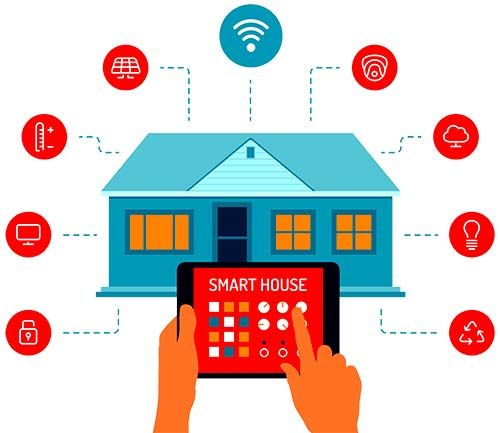
\includegraphics[width=0.8\textwidth]{./imagenes/teoria/domo.jpg} 
\caption{Sistema domótico comercial \cite{Madrid2007}.}
\label{F:domo}
\end{figure}

En la actualidad, han surgido instaladores, constructores, proyectistas, arquitectos, productores y diseñadores que han adquirido una rápida familiarización con esta tecnología  y las posibilidades que ofrecen los dispositivos, por lo que tienen el conocimiento necesario para incorporarlos y ofrecer distintos productos, en un mercado que está incrementado exponencialmente su competitividad e ingresos.
%%%------------------------------------------
\subsection{Ventajas y desventajas de un sistema domótico}
%%%------------------------------------------

Según \cite{Madrid2007}, algunas de las ventajas de un sistema de este tipo son:

\begin{itemize}
\item \textbf{Climatización y consumo energético}: se puede programar el encendido y apagado de aparatos electrónicos y luces, además de usan medidores de energía en tiempo real que informe el consumo al usuario.
\item \textbf{Entretenimiento y confort}: permite conectar el internet a los componentes de la casa, concepto que esta en tendencia con el Internet de las cosas (IoT, \textit{Internet of Things}, por sus siglas en inglés), por lo que se facilita el uso de los componentes del hogar.
\item \textbf{Seguridad}: configuración de procedimientos de avisos en caso de intrusión o avería, instalación de cámaras y micrófonos, control de acceso a la vivienda, entre otros.
\item \textbf{Comunicación}: debido al uso de redes de internet se puede tener un control remoto y tener los datos del estado del hogar desde cualquier parte.
\end{itemize}

Además algunas de las desventajas descritas en \cite{Madrid2007}, son:
\begin{itemize}
\item \textbf{Inversión inicial}: todavía resulta muy caro ya que hay que cablear toda la casa.
\item \textbf{Casas nuevas}: estos sistemas están tienen relativamente mayor exitoso en casas, ya que, en las casa viejas y que no fueron diseñadas para esta tecnología, el costo inicial se incrementa aún más. 
\item \textbf{Problemas de seguridad}: si se usa sistema domótico con control por medio de una red remota, como lo son la mayoría de los que se ofrecen comercialmente, se pueden presentar problemas de seguridad y hackeo del sistema.
\item \textbf{Falta de normativas}: debido al reciente auge de está tecnología, en muchos países, existen pocas normas que regulan la instalación de estos sistemas y no se tienen procedimientos de instalación y mantenimiento que garantice la seguridad de los ocupantes de una vivienda con un sistema domótico.
\end{itemize}

%%%------------------------------------------
\section{Servidor web}
%%%------------------------------------------

En términos sencillos un servidor web es un programa diseñado para permitir la interacción entre ordenadores.

Suele funcionar permaneciendo a la espera de peticiones. Cuando las recibe responde a ellas transfiriendo documentos de tipo hipertexto, Para ello implementa el protocolo HTTP (\textit{HyperText Transfer Protocol}, por sus siglas en inglés). En la figura \ref{F:peticion}, se ejemplifica el concepto de peticiones en un servidor web.

\begin{figure}[H]
\centering
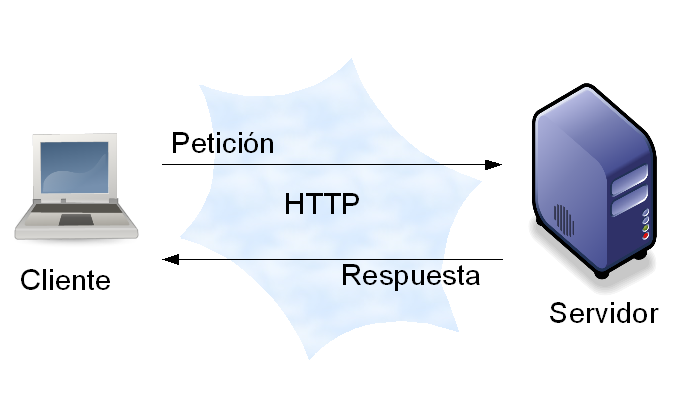
\includegraphics[width=0.55\textwidth]{./imagenes/teoria/peticion.png} 
\caption{Petición en un servidor web.}
\label{F:peticion}
\end{figure}

En donde el servidor y el cliente se encargan de:

\begin{itemize}
\item \textbf{Servidor}:
  \begin{enumerate}
  \item Espera las peticiones
  \item Envía archivos
  \item Ejecuta CGIs (en respuesta a las peticiones) y envía los resultados
  \item Establece conexión a Sistemas de Bases de Datos
  \item Actúa de puerta de enlace para servicios como el correo, ftp, etc
  \end{enumerate}
\item \textbf{Cliente}:
	\begin{enumerate}
    \item Realiza las peticiones
    \item Interpreta el código HTML que recibe
    \item Arranca aplicaciones externas.
    \item Controla aspectos del formato del documento.
	\end{enumerate}
\end{itemize}

Además es importante conocer a cerca de los requisitos mínimos para la implementación de un servidor web, los cuales según \cite{Sanchez2018} son:
\begin{itemize}
\item \textbf{Hardware}: Un ordenador tipo PC de nivel básico (2010-Pentium, 1 Gb RAM, 20 Gb HD)
\item \textbf{Software}: Programas específicos, programas para ejecutar aplicaciones, herramientas de desarrollo
\item \textbf{Conectividad}: Ordenador conectado a internet y ejecutando TCP/IP
\end{itemize}
%%%------------------------------------------
\subsection{Servidor web local}
%%%------------------------------------------

Un servidor web local es aquel que reside en una red local al equipo de referencia. El servidor web local puede estar instalado en cualquiera de los equipos que forman parte de una red local. Es por tanto obvio, que todos los servidores web, son locales a la red local en la que se encuentran, o como mínimo, locales al sistema en el que están instalados. 

En la figura \ref{F:RED}, se muestra una configuración típica de una red local, en este proyecto se van conectar los componentes electrónicos tipo Sonoff por medio de conexión Wi-Fi, al igual que componentes por ethernet, como cámaras. 

\begin{figure}[H]
\centering
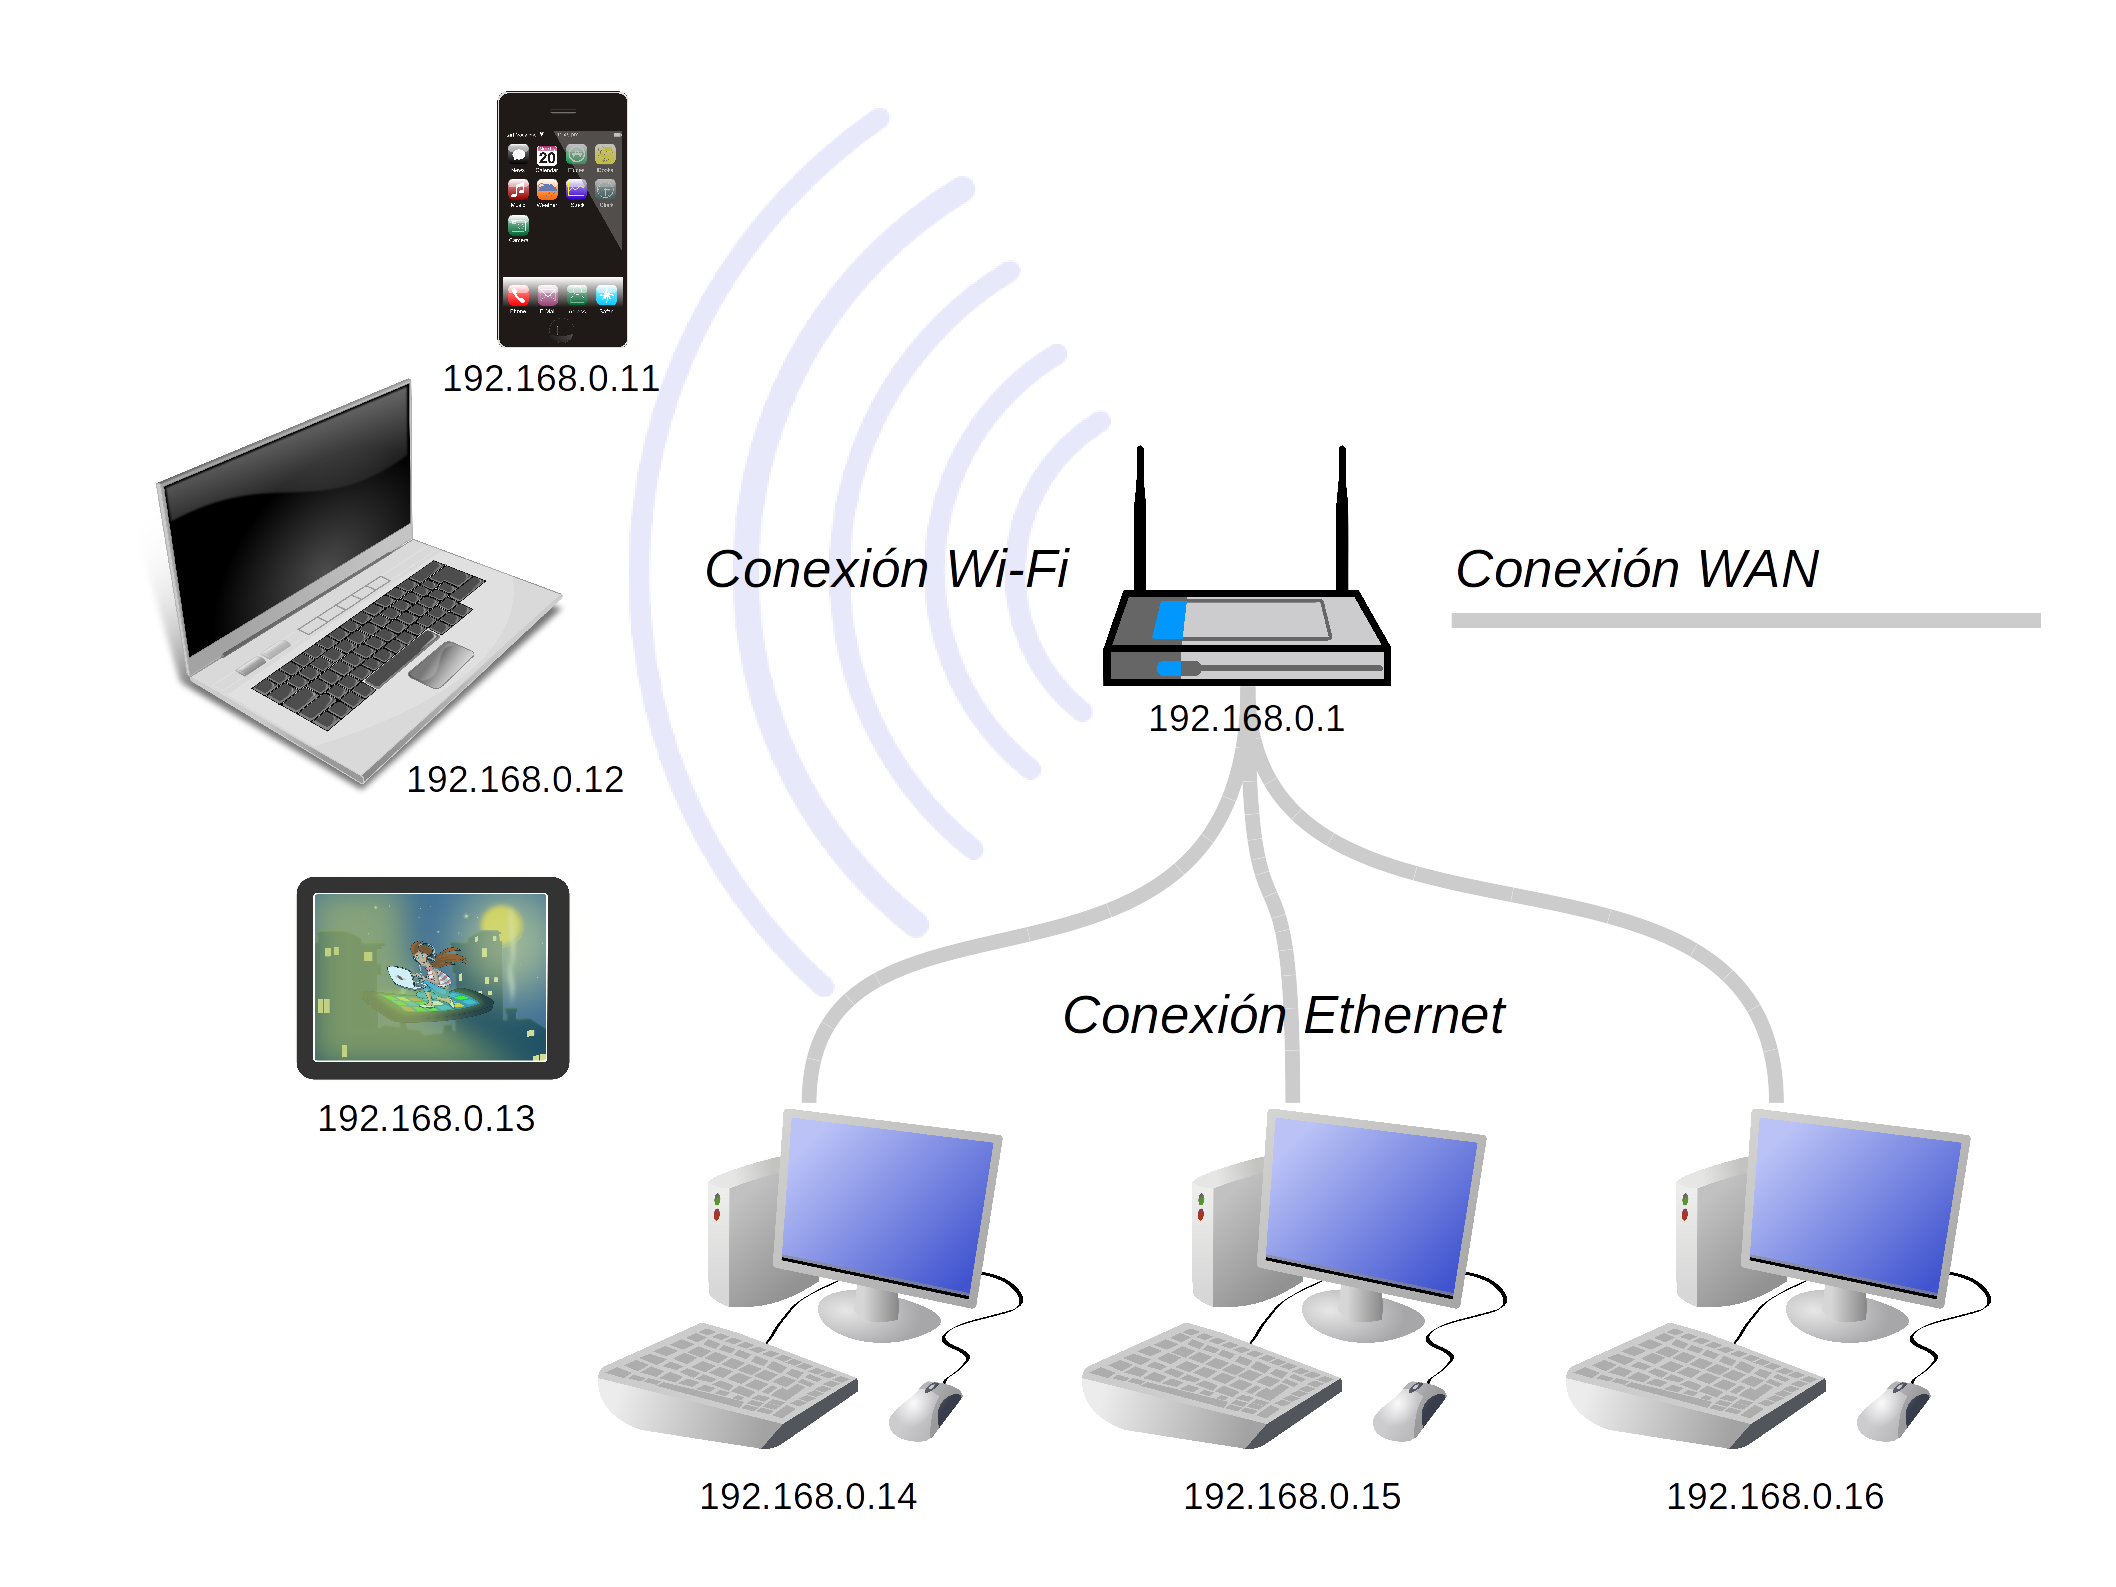
\includegraphics[width=0.8\textwidth]{./imagenes/teoria/red_local.png} 
\caption{Red local con router inalámbrico \cite{Sanchez2018}.}
\label{F:RED}
\end{figure}

Existen numerosas aplicaciones que facilitan la instalación automática de servidores web Apache y aplicaciones adicionales como MySQL y PHP (entre otros), de forma conjunta, como XAMPP, JAMP o EasyPHP. Estas aplicaciones reciben el nombre de LAMP cuando se instalan en plataformas Linux, WAMP en sistemas Windows y MAMP en sistemas Apple Macintosh.

Algunos servidores web importantes son:

\begin{itemize}
\item Nginx
\item Apache
\item Internet Information Services (IIS)
\item Cherokee
\item Tomcat
\end{itemize}

Según \cite{Sanchez2018}, entre las ventajas de un servidor web local se encuentran:

\begin{itemize}
\item Seguridad, ya que, los que acceden al servidor son los equipos conectados a una red local. 
\item Se puede hacer todo tipo pruebas a nuestro sitio sin temor a estropear el sitio, al fin y al cabo, para eso sirve el localhost.
\item No es necesario contratar un dominio (dirección) ya que es 127.0.0.1 y el disco duro funciona como el hosting (y por así decirlo es ilimitado).
\item Teniendo el sitio montado en internet, se puede tener también el localhost como respaldo.
\item Logra minimizar el número de credenciales dentro de la red.
\item Es escalable, por lo que se puede cambiar el tamaño del servidor local fácilmente en el caso de ser necesario.
\end{itemize}

Entre las principales desventajas se encuentran \cite{Sanchez2018}:
\begin{itemize}
\item Es necesario tener una computadora conectada para poder mantener el servidor local.
\item No se puede respaldar la información.
\item Alto consumo de energía y baterías limitadas en caso de fallos de luz
\item Se puede centralizar la gestión de los usuarios y las contraseñas.
\end{itemize}

%%%------------------------------------------
\subsubsection{Nginx}
%%%------------------------------------------

Es un software libre y de código abierto, licenciado bajo la Licencia BSD simplificada; también existe una versión comercial distribuida bajo el nombre de nginx plus. Es multiplataforma, por lo que corre en sistemas tipo Unix (GNU/Linux, BSD, Solaris, Mac OS X, etc.) y Windows.

\begin{figure}[H]
\centering

\includegraphics[width=0.3\textwidth]{./imagenes/teoria/nginz.png} 
\caption{Logo de la marca comercial Nginx.}
\label{F:NGINX}
\end{figure}

%%%------------------------------------------
\subsubsection{Apache}
%%%------------------------------------------
Apache es posiblemente el servidor Web más utilizado en el mundo. Todas las distribuciones Linux cuentan con un servidor Apache integrado en la propia distribución por lo cual solamente hay que seleccionar la opción de instalar el servidor para que éste quede instalado y funcional \cite{Apache2018}.

\begin{figure}[H]
\centering

\includegraphics[width=0.35\textwidth]{./imagenes/teoria/apache.png} 
\caption{Logo de la marca comercial Apache.}
\label{F:APACHE}
\end{figure}

La ventaja de estos dos software, es que se encuentran como licencia libre, lo que facilita la implementación de un servidor local en un dispositivo que corra bajo una distribución GNU/Linux. 


%%%------------------------------------------
\section{Componentes electrónicos Sonoff}
%%%------------------------------------------
El fabricante de estos producto es ITEAD, el cuál se especializa en el desarrollo y fabricación de hardware y productos para el hogar inteligente. Ubicada en Shenzhen, el mercado electrónico más grande de China y la cadena de suministro electrónico más integrada del mundo, lo que permite ofrecer productos innovadores de alta calidad a bajo costo \cite{Sonoff2018}. En la figura \ref{F:sonoff}, se puede ver un ejemplo de uso de estos componentes y como es que se ve una posible instalación de este sistema.

\begin{figure}[H]
\centering
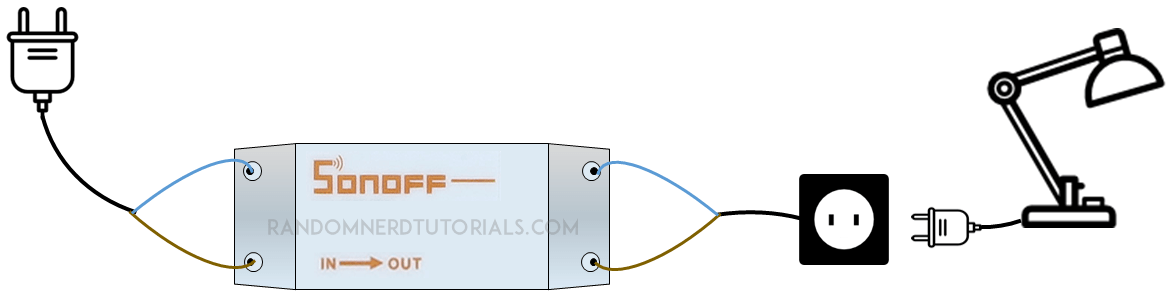
\includegraphics[width=\textwidth]{./imagenes/teoria/SONOFF_circuit.png} 
\caption{Ejemplo de componente domótico \cite{Sonoff2018}.}
\label{F:sonoff}
\end{figure}

Entre las ventajas de estos componentes, es el precio, que ronda entre \$4 - \$20, por lo que son relativamente baratos. Además, como se mencionó en el capítulo anterior, una de las principales ventajas de estos componentes es que permiten la ingeniería inversa. Este concepto consiste en recuperar el diseño de una aplicación o producto a del partir del código o diagramas que ayudan a entender el funcionamiento del componente. El objetivo de la ingeniería inversa es obtener información a partir de un producto accesible al público, con el fin de determinar de qué está hecho, qué lo hace funcionar y cómo fue fabricado. Está característica en lo componentes Sonoff es de vital importancia, ya que, nos permite editar la configuración por defecto de los componentes y adaptarlos para que se comporten de una manera distinta, en nuestro caso esta configuración se hará para realizar la conexión a una red local. 
 
Existen una gran variedad de componentes de esta compañía, a continuación en la tabla \ref{T:Sonoff}, se muestran algunas de las características básicas de cada uno de los componentes Sonoff.

\begin{table}[H]
\centering
\caption{Descripción de los componentes electrónicos Sonoff \cite{Sonoff2018}.} \label{T:Sonoff}
\begin{tabular}{ | >{\centering\arraybackslash}m{2.5cm} | >{\centering\arraybackslash}m{12cm}  | }
    \hline
    \cellcolor{cl} \textbf{Componente} & \cellcolor{cl} \textbf{Funcionamiento}  \\
    \hline
    \hline
    Sonoff Basic & Es un interruptor con conexión Wi-Fi, que se puede programar para que funcione en horas específicas, con operación de \SI{90}{\volt} - \SI{250}{\volt} en AC y capacidad de corriente máxima de \SI{10}{A}.\\ \hline
    Sonoff RF & Cumple con las mismas funciones que el Sonoff Basic, con la diferencia de que se puede utilizar por medio de una infrarroja de \SI{433}{MHz}. \\ \hline
    Sonoff TH10/TH16 & Permite medir la temperatura y la humedad, haciendo uso de sensores de alta precisión.  \\ \hline
    Sonoff Dual & Cumple con funciones similares al Sonoff Basic, con la diferencia de que se pueden utilizar dos cargas y manejarse de manera independiente cada una de ellas. \\ \hline
    Sonoff Pow & Permite el monitoreo del consumo de energía en tiempo real, con operación de \SI{90}{\volt} - \SI{250}{\volt} en AC, capacidad de corriente máxima de \SI{10}{A} y de potencia de \SI{3500}{W}.\\ \hline
    Sonoff 4CH & Básicamente son 4 relés con monitoreo del consumo de energía y que se pueden programar los horarios de operación de los componentes, con operación de \SI{90}{\volt} - \SI{250}{\volt} en AC, capacidad de corriente máxima de \SI{10}{A} y de potencia máxima de \SI{2200}{W}. \\ \hline
    Sonoff G1 & Cumple con las mismas funciones que el Sonoff Basic, con la diferencia de que se puede utilizar por medio de GPRS al conectarle una tarjeta SIM, lo que lo hace ideal para aplicaciones en el área agrícola o en jardines.  \\ \hline 
    Sonoff Pow R2 & Está versión permite monitorear en tiempo real no solo el consumo de energía, sino la tensión y la corriente, además se puede programar para que actué como protección a sobrecargara al poder configurar un valor máximo de carga y se puede generar un registro de los datos.  \\ \hline
    Sonoff 4CH PRO & Similar a la versión 4CH, pero con capacidad de ser utilizado con una señal infrarroja de \SI{433}{MHz} y bloque de los relés.   \\ 
    \hline
\end{tabular}
\end{table}

En la figura \ref{F:PRODUCTS}, se puede observar el diseño físico de cada uno de los componentes descritos en la tabla anterior.

\begin{figure}[H]
\centering
\begin{tabular}{c c c}

\subfloat[Basic]
{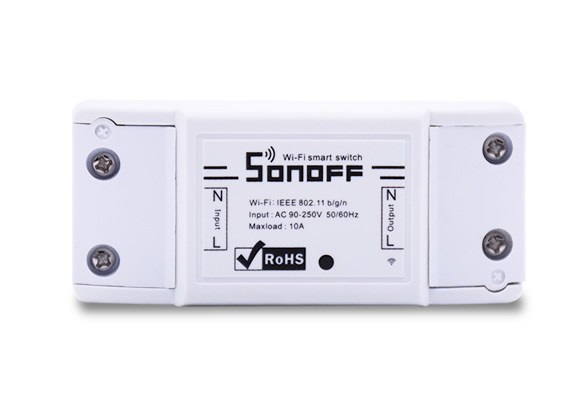
\includegraphics[width=0.33\textwidth]{./imagenes/teoria/BASIC.jpg}}
&
\subfloat[RF]{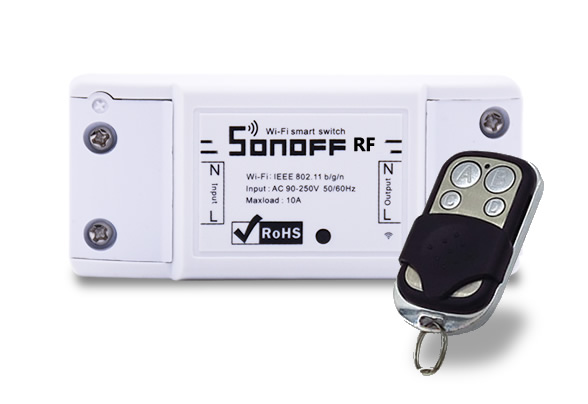
\includegraphics[width=0.33\textwidth]{./imagenes/teoria/RF.jpg} }
&
\subfloat[TH10/TH16]{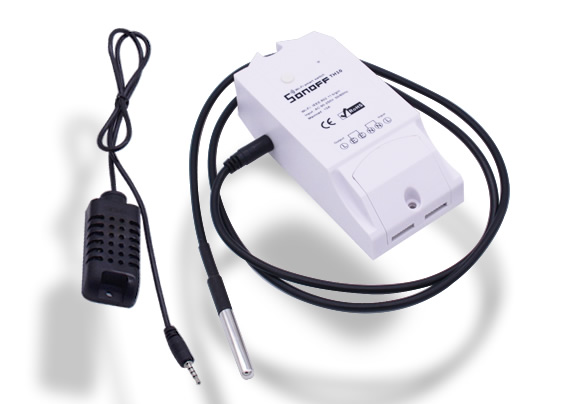
\includegraphics[width=0.33\textwidth]{./imagenes/teoria/TH1.jpg} }
\\

\subfloat[G1]
{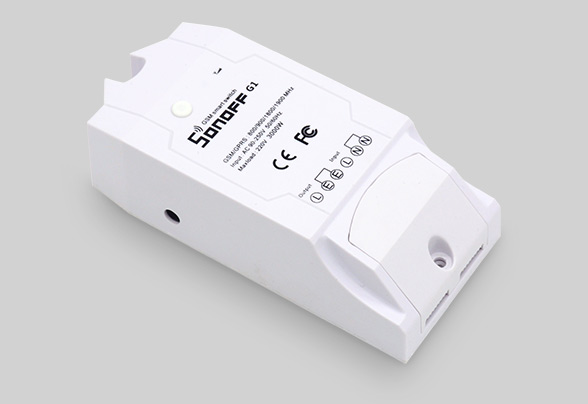
\includegraphics[width=0.33\textwidth]{./imagenes/teoria/G1.jpg}}
&
\subfloat[4CHPRO]{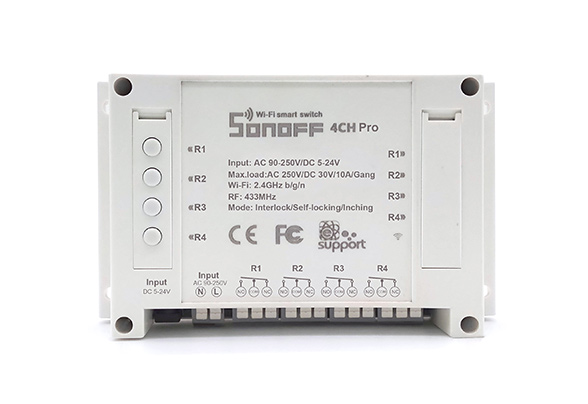
\includegraphics[width=0.33\textwidth]{./imagenes/teoria/4CHPRO.jpg} }
&
\subfloat[Pow R2]{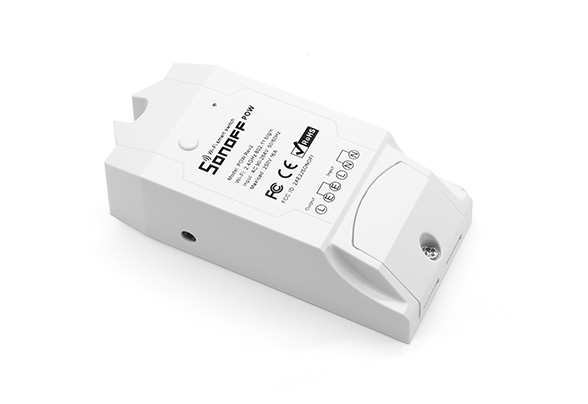
\includegraphics[width=0.33\textwidth]{./imagenes/teoria/POWR2.jpg} }
\\

\subfloat[Dual]
{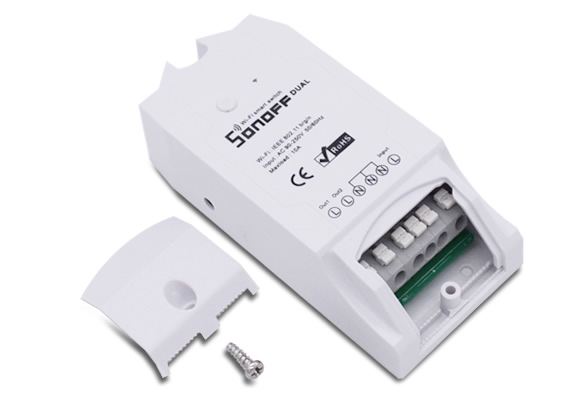
\includegraphics[width=0.33\textwidth]{./imagenes/teoria/DUAL.jpg}}
&
\subfloat[Pow]{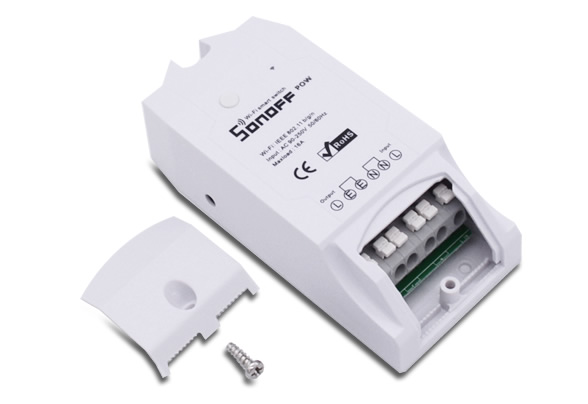
\includegraphics[width=0.33\textwidth]{./imagenes/teoria/POW.jpg} }
&
\subfloat[4CH]{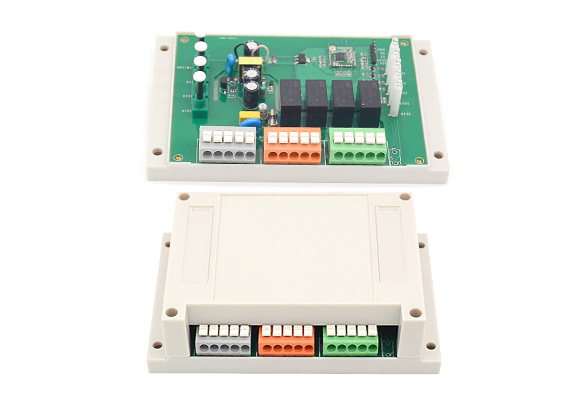
\includegraphics[width=0.33\textwidth]{./imagenes/teoria/4CH.jpg} }
\\

\end{tabular}
\caption{Componentes electrónicos Sonoff.}
\label{F:PRODUCTS}
\end{figure}


%%%------------------------------------------
\subsection{Reprogramación de los componentes Sonoff}
%%%------------------------------------------

Como se menciono anteriormente, una de las principales ventajas de estos componentes es que se pueden editar la configuración por defecto de los mismos. Estos componentes se pueden abrir y realizar la configuración de pines para conectar por comunicación serial haciendo uso de un módulo de conexión USB.

Una vez realizada está configuración, se puede editar usando el \textit{Arduino IDE}, el cual es un software de código abierto, que hace que sea fácil escribir código y subirlo a la tarjeta. Se ejecuta en Windows, Mac OS X y Linux. El entorno está escrito en Java y está basado en \textit{Processing} y otro software de código abierto. A la hora de programación tiene una sintaxis lingüística muy similar a la de C \cite{Arduino2018}. 

\begin{figure}[H]
\centering
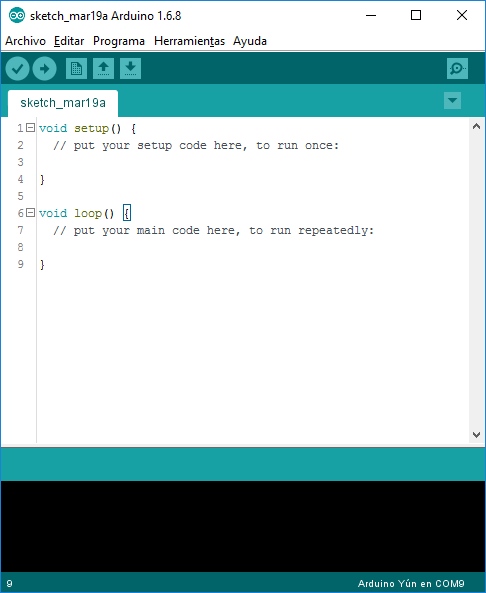
\includegraphics[width=0.8\textwidth]{./imagenes/teoria/ide.png} 
\caption{Interfaz del Arduino IDE \cite{Arduino2018}.}
\label{F:IDE}
\end{figure}



%%%------------------------------------------
\section{Interfaces de usuario}
%%%------------------------------------------

Las interfaces de usuario, son la parte de programa o aplicación que interactúa con un usuario para realizar tareas específicas.

Douglas Engelbart, además de inventor del ratón de ordenador, desarrolló la primera interfaz gráfica en los años 1960 en EE.UU. en los laboratorios de XEROX. Fue introducida posteriormente al público en las computadoras Apple Macintosh en 1984, y a las masas hasta 1993 con la primera versión popular del sistema operativo Windows 3.0

En la actualidad, el uso de interfaces de usuario se encuentra en diversas áreas debido a sus facilidad de interacción con el usuario, por lo que hoy día lo podemos ver en cualquier tipo de componentes, como celulares, microondas, cocinas, lavadoras, carros, televisores, aires acondicionados, radios, aviones, entre muchos otros ejemplos más. Por lo tanto, La historia reciente de la informática está indisolublemente unida a las interfaces gráficas, puesto que los sistemas operativos gráficos han ocasionado grandes consecuencias en la industria del software y del hardware \cite{Pavon2017}. Las interfaces de usuario se han divido en tres áreas fundamentales, las cuales son:

\begin{itemize}
\item \textbf{CLI} : La interfaz de línea de comandos (\textit{Command Line Interface}, por sus siglas en inglés), es un método que permite a los usuarios dar instrucciones a algún programa informático por medio de una línea de texto simple, actualmente conocido como Terminal o Bash.
\item \textbf{GUI} : La interfaz gráfica de usuario (\textit{Graphical User Interface}, por sus siglas en inglés)  es un método para facilitar la interacción del usuario con el ordenador o la computadora a través de la utilización de un conjunto de imágenes y objetos pictóricos (iconos, ventanas...) además de texto. Surge como evolución de la línea de comandos de los primeros sistemas operativos y es pieza fundamental en un entorno gráfico \cite{Pavon2017}.

\item \textbf{NUI} : La interfaz natural de usuario (\textit{Natural User Interface}, por sus siglas en inglés), según \cite{Pavon2017}, en este tipo el usuario interactúa con un sistema, aplicación, etcétera, sin utilizar sistemas de mando o dispositivos de entrada (como en las interfaces gráficas de usuarios, sería un ratón, teclado alfanumérico, lápiz óptico, panel táctil, joystick, etcétera), y en su lugar, se hace uso de movimientos gestuales del cuerpo o de alguna de sus partes tales como las manos, sirviendo de mando de control.
\end{itemize}

A continuación en la figura \ref{F:GUI}, se puede apreciar una imagen que ejemplifica de mejor manera esta clasificación.

\begin{figure}[H]
\centering
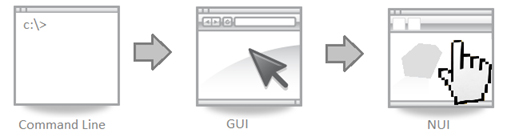
\includegraphics[width=\textwidth]{./imagenes/teoria/gui.jpg} 
\caption{Tipos generales de interfaces gráficas.}
\label{F:GUI}
\end{figure}

Para este proyecto, se hará especial énfasis a las GUI, ya que, es lo que  se desea diseñar en este proyecto, aunque en la actualidad la surgido una gran tendencia en el área de sistemas domóticos a usar interfaces de usuario tipo NUI, debido a que facilita el uso celulares y tablets. 

Debido al amplio uso de las GUI en tantas diversas áreas existen varios lenguajes de programación y herramientas para el diseño de interfaces gráficas, a continuación se presentan los principales:

\begin{itemize}
\item Python.
\item Glade.
\item Java (AWT  y Swing).
\item QT5.
\item Visual Basic.
\item WXWINDOWS.
\end{itemize}

Además existen varios principios que se usan para el diseño de interfaces gráficas de manera correcta, se manejan los siguientes conceptos:

\begin{itemize}
\item Sencilla
\item Flexible
\item Coherente
\item Autonomía
\item Percepción del color
\item Legibilidad 
\end{itemize}

%%%------------------------------------------
\subsection{Desarrollo de interfaces con QT5}
%%%------------------------------------------

Según \cite{QT52018}, se dice Qt es un framework multiplataforma orientado a objetos ampliamente usado para desarrollar programas (software) que utilicen interfaz gráfica de usuario, así como también diferentes tipos de herramientas para la línea de comandos y consolas para servidores que no necesitan una interfaz gráfica de usuario.

En 1991, Haavard Nord y Eirik Chambe-Eng, inician el desarrollo de QT, desde ese entonces a formado parte de la plataforma usada por grandes compañías a nivel mundial para el diseño de interfaces, empezando desde el 2001 con Nokia. En Marzo 2011, se publicó una versión, en el cuál se inicia la compatibilidad con Android, iOS, Linux y la plataforma de Windows. En la figura \ref{F:qt5}, se muestra el logo que representa la marca. 

\begin{figure}[H]
\centering

\includegraphics[width=0.3\textwidth]{./imagenes/teoria/qt5.jpg} 
\caption{Logo de la marca comercial QT5. \cite{QT52018}}
\label{F:qt5}
\end{figure}

Entre sus principales características se encuentra que:

\begin{itemize}
\item Es de software libre y código abierto.
\item El lenguaje de programación es C++, de forma nativa, adicionalmente puede ser utilizado en varios otros lenguajes de programación a través de \textit{bindings} \footnote{\textbf{Bindings}: es una adaptación de una biblioteca para ser usada en un lenguaje de programación distinto de aquel en el que ha sido escrita.}.
\item Usa un lenguaje declarativo, por lo que se describe el aspecto de los elementos y se centra en interfaces gráficas.
\item Una de las ventajas de usar esta herramienta, es que debido a su auge en los últimos años, se encuentran disponibles en línea varios manuales, foros y tutoriales que ayudan al uso de la plataforma. 
\end{itemize}

Es ampliamente usado por la industria de sistemas embedidos y empresas como: Agencia Espacial Europea, DreamWorks, Lucasfilm, Panasonic, Philips, Samsung, Siemens AG, Volvo, Walt Disney Animation Studios, Blizzard Entertainment, Electronic Arts, AMD, Research In Motion, HP, entre otros; hacen uso de este software para el desarrollo de las interfaces gráficas para sus productos. Para el caso del diseño de interfaces para sistemas domóticos usando esta herramienta, en la actualidad ya se han realizado proyectos de esta índole, por lo que en este proyecto se propone usar manuales de referencia. En la figura \ref{F:homeqt5}, se muestra un ejemplo del diseño de una interfaz con este software.

\begin{figure}[H]
\centering
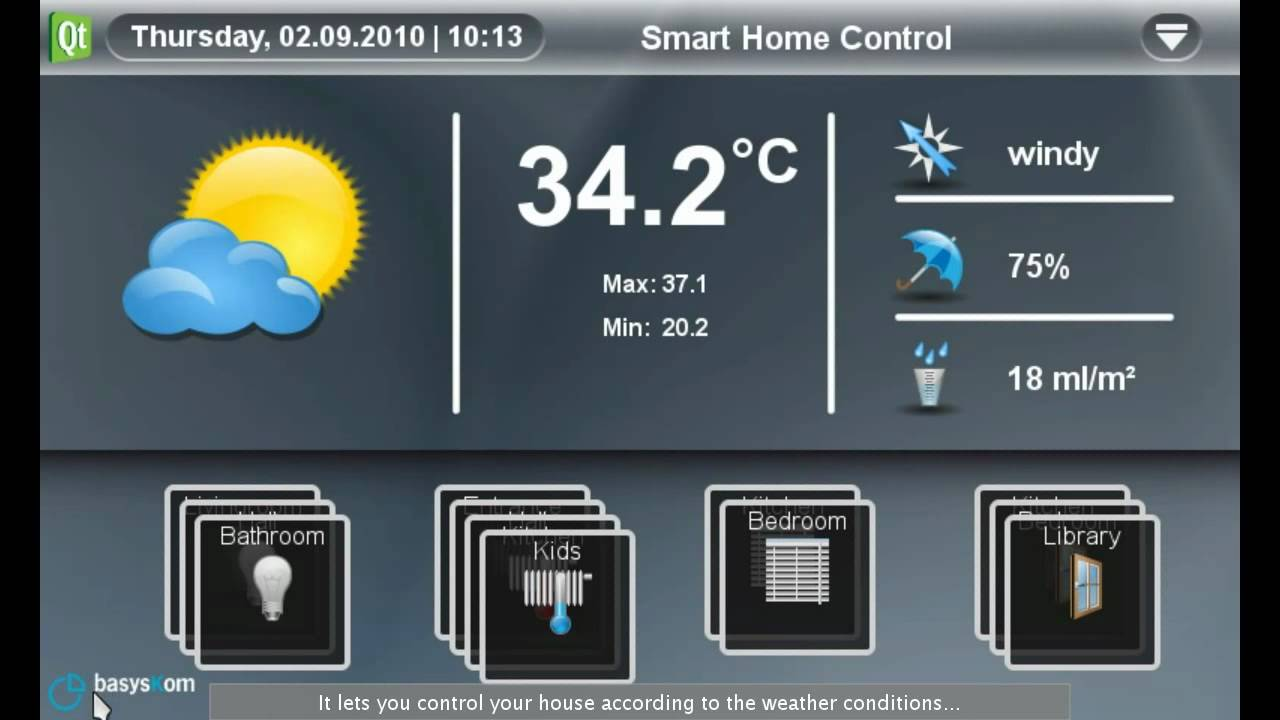
\includegraphics[width=0.8\textwidth]{./imagenes/teoria/homeqt.jpg} 
\caption{Ejemplo de interfaz para sistemas domótico diseñado con QT5. \cite{QT52018}}
\label{F:homeqt5}
\end{figure}




%\input{contenido/3_mecanum.tex}
%\input{contenido/4_modelodcpid.tex}
%\input{contenido/5_modelocine.tex}
%\input{contenido/6_odonav.tex}
%\input{contenido/7_move.tex}
%\input{contenido/8_conclusiones.tex}

% 8. BILIOGRAFÍA
\bibliographystyle{plain}
\bibliography{bibliografia/bibliografia.bib}

% 9. APÉNDICES
\appendix
\chapter{Cronograma de actividades a desarrollar}

A continuación en la tabla \ref{T:Scheduler}, se muestra un resumen del cronograma de actividades a desarrollar.

\begin{table}[H]
\centering
\caption{Cronograma de desarrollo de actividades} \label{T:Scheduler}
\begin{tabular}{ | >{\centering\arraybackslash}m{6cm} | >{\centering\arraybackslash}m{4cm}  >{\centering\arraybackslash}m{4cm} | }
    \hline
    \cellcolor{cl} \textbf{Actividad} & \cellcolor{cl} \textbf{Mes} & \cellcolor{cl} \textbf{Semana} \\
    \hline
    \hline
    \multirow{5}{6cm}{\centering  Etapa de desarrollo del servidor local} 
    						  & Agosto & Semana 2 \\ \cline{2-3}
    						  & Agosto & Semana 3 \\ \cline{2-3}
                              & Agosto & Semana 4 \\ \cline{2-3}
                              & Septiembre & Semana 1 \\ \cline{2-3}
							  & Septiembre & Semana 2 \\ \hline
    \multirow{7}{6cm}{\centering  Etapa de integración de los componentes electrónicos tipo Sonoff} 
    						  & Septiembre & Semana 3 \\ \cline{2-3}
    						  & Septiembre & Semana 4 \\ \cline{2-3}
                              & Octubre & Semana 1 \\ \cline{2-3}
                              & Octubre & Semana 2 \\ \cline{2-3}
                              & Octubre & Semana 3 \\ \cline{2-3}
                              & Octubre & Semana 4 \\ \cline{2-3}
							  & Noviembre & Semana 1 \\ \hline 
    \multirow{7}{6cm}{\centering Etapa de diseño de la interfaz gráfica} 
    						  & Noviembre & Semana 2 \\ \cline{2-3}
    						  & Noviembre & Semana 3 \\ \cline{2-3}
                              & Noviembre & Semana 4 \\ \cline{2-3}
                              & Diciembre & Semana 1 \\ \cline{2-3}
                              & Diciembre & Semana 2 \\ \cline{2-3}
                              & Enero & Semana 2 \\ \cline{2-3}
							  & Enero & Semana 3 \\ \hline  
    \multirow{5}{6cm}{\centering Etapa de validación} 
    						  & Enero & Semana 4 \\ \cline{2-3}
    						  & Febrero & Semana 1 \\ \cline{2-3}
                              & Febrero & Semana 2 \\ \cline{2-3}
                              & Febrero & Semana 3 \\ \cline{2-3}
							  & Febrero & Semana 4 \\ \hline 
    \multirow{3}{6cm}{\centering Redacción del reporte final } 
    						  & Marzo & Semana 1 \\ \cline{2-3}
    						  & Marzo & Semana 2 \\ \cline{2-3}
                              & Marzo & Semana 3 \\ \hline 
    \multirow{3}{6cm}{\centering Revisión profesor guía y lectores} 
    						  & Marzo & Semana 4 \\ \cline{2-3}
    						  & Abril & Semana 1 \\ \cline{2-3}
                              & Abril & Semana 2 \\ \hline                          
\end{tabular}
\end{table}

%\input{apendices/B_video.tex}
%\input{apendices/B_gopro.tex}
%\input{apendices/C_codes.tex}
%\input{apendices/D_connection.tex}

\backmatter



%%%%%%%%%%%%%%%%%%%
\end{document}
%%%%%%%%%%%%%%%%%%%
